\documentclass[12pt,a4paper]{article}
\usepackage[utf8]{inputenc}
\usepackage[a4paper,vmargin={20mm,20mm},hmargin={10mm,10mm}]{geometry}
\usepackage{amsmath}
\usepackage{amssymb}
\usepackage{mathtools}
\usepackage{enumitem}
\usepackage{graphicx}
\usepackage{scrextend}
\usepackage{blindtext}
\usepackage{caption}
\usepackage{url}
\usepackage{subcaption}
\usepackage{circuitikz}
\usepackage{listings}
\usepackage{color}
\usepackage{bbm}
\usepackage{stmaryrd}
\usepackage{booktabs}
\usepackage{array}
\usepackage{tablefootnote}
\usepackage{algorithmicx}
\usepackage{algorithm}
\usepackage{algpseudocode}
\usepackage{blkarray}
\usepackage{tikz}
\usepackage{subfig}
\usepackage{tcolorbox}
\usepackage{xcolor}

\definecolor{codegreen}{rgb}{0,0.6,0}
\definecolor{codegray}{rgb}{0.5,0.5,0.5}
\definecolor{codepurple}{rgb}{0.58,0,0.82}
\definecolor{backcolour}{rgb}{0.95,0.95,0.92}
 
\lstdefinestyle{mystyle}{
    backgroundcolor=\color{backcolour},   
    commentstyle=\color{codegreen},
    keywordstyle=\color{magenta},
    numberstyle=\tiny\color{codegray},
    stringstyle=\color{codepurple},
    basicstyle=\footnotesize,
    breakatwhitespace=false,         
    breaklines=true,                 
    captionpos=b,                    
    keepspaces=true,                 
    numbers=left,                    
    numbersep=5pt,                  
    showspaces=false,                
    showstringspaces=false,
    showtabs=false,                  
    tabsize=2
}
 
\lstset{style=mystyle}
 
\newcommand*{\QEDB}{\hfill\ensuremath{\square}}% 

\definecolor{lightblue}{RGB}{46,164,215}
\definecolor{darkblue}{RGB}{11,124,174}
\definecolor{darkdarkblue}{RGB}{7,101,142}
\definecolor{fiordalisoblu}{RGB}{171, 205, 239}

\tcbset{colback=white,colframe=fiordalisoblu,fonttitle=\sffamily, boxrule=0.2mm}
\newcommand*\rot{\rotatebox{90}}
\newcommand{\twolinecell}[2][c]{%
  \begin{tabular}[#1]{@{}c@{}}#2\end{tabular}}

\DeclarePairedDelimiter\floor{\lfloor}{\rfloor}
\begin{document}
\title{\textbf{Algorithmic Methods for Mining Large Graphs}}
\author{Marco Ponza\\Department of Computer Science\\University of Pisa\\\texttt{marco.ponza@di.unipi.it}}
%\date{\today}
\maketitle

\section*{Terminology}
When not specify, we use the following terminology. A graph $G = (V, E)$ is a pair of two sets: $V$, the set of nodes, and $E$, the set of edges, with $n = |V|$ and $m = |E|$. Edges are undirected and unweighted.


\section*{Exercise 1}

\begin{description}

\item[Citation Network: Directed and Acyclic.] Since the model citation networks can be modeled as a graph, we expect that it is directed by construction: articles are nodes and a directed edge between two nodes $(u, v)$ represents that article $u$ cites article $v$. Clearly, there is no cylces under the assumption that articles have only ``older'' references respect their publication date.

\item[Citation Network: Small Cycles.] On the other hand, a cycle can be generated when we have two (or more) groups of researchers that are collaborating on two (or more) distinct papers (which cite each other) and they are published in the same conference/journal. However, since this is not common, we can expect that our graphs will contain a relative small amount of cycles.

\item[Cycle Detection.] In order to detect if a citation network is cyclic, we can deploy Algorithm \ref{algo:cycle} (see \textsc{CycleDetection} procedure). Specifically, $graph$ is the directed adjacency lists of our graph, where keys are nodes and values are the corresponding out-edges (list of nodes), and $state$ is a data structure that assigns a state to each node in the graph: ``not yet visited'' (value 0), ``visiting'' (value 1) and ``visited'' (value 2). A cycle is detected when, during the DFS-visit, we encounter a node that we are already visiting. Both $graph$ and $state$ are used in the pseudocode as Python dictionary. The worst case running time is $\mathcal{O}(n + m)$: $\mathcal{O}(n)$ is the time to set all entries of $state$ to 0 and $\mathcal{O}(m)$ is due to DFS procedure, where each edge is visited once.



\begin{algorithm}
\caption{Cycle Detection via DFS.}\label{algo:cycle}
\begin{algorithmic}[1]
\Function{CycleDFS}{$node, graph, state$}
\State $state[node] \gets 1$
\ForAll{$out \in graph[node]$}
    \If {$state[out] = 1$}
    	\State \Return True
    \ElsIf {$state[out] = 0$}
        \If {CycleDFS($out, graph, state$)}
        	\State \Return True
\algstore{myalgo}
\end{algorithmic}
\end{algorithm}

\begin{algorithm}
\addtocounter{algorithm}{-1}
\caption{Cycle Detection via DFS (continued).}
\begin{algorithmic}[1]
\algrestore{myalgo}
        \EndIf
    \EndIf
\EndFor
\State $state(node) \gets 2$
\State \Return False
\EndFunction
\State
\Function{CycleDetection}{$graph$}
\ForAll{$node \in graph$}
	\State $state[node] \gets 0$
\EndFor
\ForAll{$node \in graph$}
	\If {$state[node] = 0$}
    \If {\textsc{CycleDFS}($node, graph, state$)}
    	\State \Return ``Your graph is cyclic!''
    \EndIf
    \EndIf
\EndFor
\State \Return ``Your graph is acyclic!''
\EndFunction
\end{algorithmic}
\end{algorithm}

\end{description}



\section*{Exercise 2}
We indicate the adjacent list of the node $u$ as $adj\_list(u)$ (list of nodes linked to $u$): in the pseudocode, we will use it as a Python list. The detailed algorithm which uniformly samples triplets can be found in the following pseudocodes (Algorithms ~\ref{algo:first}, \ref{algo:second}, \ref{algo:third}). Specifically, for each step, we will report the pseudocode and its description.

\begin{algorithm}
\caption{First step of the three-pass algorithm.}\label{algo:first}
\begin{algorithmic}[1]
\Function{TripletCounting}{$stream$}
\State $c \gets 0$
\ForAll{$adj\_list(u) \in stream$}
	\State $triplets \gets |adj\_list(u)| \cdot (|adj\_list(u)| - 1) / 2$
    \State $c \gets c + triplets $
\EndFor
\State \Return c
\EndFunction
\end{algorithmic}
\end{algorithm}

The first pass of our algorithm (Algorithm \ref{algo:first}) is performed by counting the number of triplets that can be generated by each node $u$ and its adjacent list $adj\_list(u)$. Clearly, if we denote the degree of $u$ as the cardinality of its adjacent list $|adj\_list(u)| = n$, the number of triplets that can be generated is:
\begin{align}
\dbinom{n}{2} = \frac{n!}{2! (n - 2)!} = \frac{n \cdot (n - 1)}{2}.
\end{align}


\begin{algorithm}
\caption{Second step of the three-pass algorithm.}\label{algo:second}
\begin{algorithmic}[1]
\Function{ChooseTriplet}{$stream$}
\State $r \gets \textsc{RandomNumber}(1, c)$  // $c$ computed from \textsc{TripletCounting}
\State $size \gets 0$
\ForAll{$adj\_list(u) \in stream$}
\State $size \gets |adj\_list(u)|$
\State $i \gets 0$ // index of the current node in the adjacent list
\State $prev \gets 0$ // number of encountered pairs
\ForAll{$v \in adj\_list(u)$}
	\State $l \gets prev + 1$
    \State $g \gets size + prev - i - 1$
    \If{$ r \geq l$ and $r \leq g$}
    	\State $w \gets adj\_list(u)[r - prev + i]$
    	\State \Return $(u,\ v,\ w)$
    \EndIf
    \State $prev \gets g$
    \State $i \gets i + 1$
\EndFor
\State $r \gets r - size \cdot (size - 1) / 2$
\EndFor
\EndFunction
\end{algorithmic}
\end{algorithm}
\newpage
The second step of our algorithm can be found in Algorithm \ref{algo:second}. First, we generate the random number $r$ in the range between $[1, c]$, where $c$ is the number of triplets computed by the first pass (Algorithm \ref{algo:first}). Then, we perform the second pass in order to extract the $r$-th triplet.

The rational behind this second step (Algorithm \ref{algo:second}) can be easily understood with an example. Let us assume that $r = 4$ and the input stream has only one element $v_1: [v_2, v_3, v_4, v_5]$, which is the adjacent list of the vertex $v_1$ (where $adj_list(u)[0] = v_2$, $adj_list(u)[1] = v_3$, \dots). Here, we can have 6 connected triplets:

\begin{table}[h]
\centering
\begin{tabular}{cccccc}
$(v_2, v_3)$, & $(v_2, v_4)$, & $(v_2, v_5)$, & $(v_3, v_4)$, & $(v_3, v_5)$, & $(v_4, v_5)$\\
 1 & 2 & 3& 4 & 5 & 6
\end{tabular}
\end{table}

where pairs represent triplets (we remember $v_1$ is linked to all these nodes) and the integers represent the indices that identify a triplet. Equivalently, 
we can simply re-write the pair set in matrix form, where elements are the identifiers of the triplets (pairs):

 \[
\begin{blockarray}{cccccc}
& v_2 & v_3 & v_4 & v_5 \\
\begin{block}{c(ccccc)}
  v_2 & 0 & 1 & 2 & 3   \\
  v_3 & 0 & 0 & 4 & 5   \\
  v_4 & 0 & 0 & 0 & 6  \\
\end{block}
\end{blockarray}
 \]
 
By using this matrix we can find the $r$-th triplet, but the time complexity of its construction is $\mathcal{O}(n^2)$, where $n = |adj\_list(v_1)|$. On the other hand, looking at the matrix, we can notice that a vertex $v_i$ is paired only with all vertices $v_j$, with $j > i$. Additionally, we can associate to each vertex an interval which represents the corresponding matrix row:
\begin{center}
$v_2 \rightarrow [1, 3]$\\
$v_3 \rightarrow [4, 5]$\\
$v_4 \rightarrow [6, 6]$
\end{center}

Given a random edge, we can find the corresponding vertex pair as follows. If the random triplet number is $r$, we scan each element $v_i \rightarrow [l, g]$ until we have $r \in [l, g]$. Then, the returned pair will be represented by $v$ and by the corresponding vertex of the $r$-th edge. The last vertex can be computed by ``playing'' with the indices (line 12).

We designed Algorithm \ref{algo:second} as follows. We scan the adjacency list (input of the strem) and, for each vertex $v$ (at each iteration of row 8), we assign an index $i$ and an interval, represented by $l$ and $g$ (lines 9 and 10). For each interval, we need only to check $l \leq r \leq g$. If the condition is satisfied, we compute the corresponding vertex $w$ (line 12), which is the node paired with $v$ ($r$-th triplet). Finally, we return $(u, v, w)$, where $u$ is the ``owner'' of the adjacency list.




\begin{algorithm}
\caption{Third step of the three-pass algorithm.}\label{algo:third}
\begin{algorithmic}[1]
\Function{Triangularization}{$stream$}
\State $\beta \gets \text{False}$
\ForAll{$adj\_list(z) \in stream$}
\If{$z = v$ and $w \in adj\_list(z)$ or $z = w$ and $v \in adj\_list(z)$}
\State $\beta \gets \text{True}$
    \EndIf
\EndFor
\State \Return $\beta$
\EndFunction
\end{algorithmic}
\end{algorithm}

Supposing that $(u, v, w)$ is the sample triplet, in the last pass (Algorithm \ref{algo:third}) we check if $adj\_list(v)$ (or $adj\_list(w)$) contains $w$ (or $v$). Namely, if $v$ and $w$ are connected.


\section*{Exercise 3}


\begin{description}

\item[Excact Diameter Computation.] We assume that the graph has  exactly one connected component (which can be easily checked via \textsc{BFS}-visit\footnote{If a BFS-visit from a random node does not reach $n$ nodes, the graph has more than one connected component.}): if not, the diameter will be $+\infty$.

The exact diameter of a graph can be computed by taking the maximum of the shortest distances between all pairs of vertices of a graph (Algorithm~\ref{algo:diameter}). Since we are working on undirected and unweighted graphs, BFS computes the shortest path between a node $u$ and the others.

\begin{algorithm}
\caption{Exact diameter computation.}\label{algo:diameter}
\begin{algorithmic}[1]
\Function{Diameter}{$graph$}
\State $diameter \gets 0$
\ForAll{$u \in graph$}
\State $max\_dist \gets \textsc{BFS-tree}(u,\ graph).height$
\State $diameter \gets \textsc{max}(diameter,\ max\_dist)$
\EndFor
\State \Return $d$
\EndFunction
\end{algorithmic}
\end{algorithm}
$\textsc{BFS-tree}(u, graph)$ is a function that computes a tree of a BFS-visit rooted in $u$.
\begin{itemize}

\item \textit{Running Time.} The \textsc{BFS}-visit takes $\mathcal{O}(n + m)$ time: since we have to compute it for each node in the graph, the whole running time is  $\mathcal{O}(n(n + m))$.

\end{itemize}


\item[Approximated Diameter Computation.] We can use the Flajolet-Martin sketching scheme to compute the approximated size of the diameter (Algorithm~\ref{algo:approxdiameter}) by taking inspiration from the ANF algorithm \cite{palmer2002anf}.


\begin{algorithm}
\caption{Approximated diameter computation via Flajolet-Marti sketches.}\label{algo:approxdiameter}
\begin{algorithmic}[1]
\Function{ApproximatedDiameter}{$graph$}

  \ForAll{$u \in graph.nodes$}
  	\State $B_{cur}(u).init()$
  \EndFor
  
  \For{$d \gets 1$ to $+\infty$}
  
    \ForAll{$u \in graph.nodes$}
      \State $B_{last}(u) = B_{cur}(u)$
    \EndFor
 
    \ForAll{$(u,\ v) \in graph.edges$}
    \State $B_{cur}(u) =  B_{cur}(u)\ |\  B_{last}(v)$
    \EndFor
    \State $s \gets 0$
    \ForAll{$u \in graph.nodes$}
    	\State $s \gets s + B_{cur}(u).count()$
    \EndFor
    
    \If{${|graph.nodes|}^2 - s < \epsilon$}
    	\State \Return $d$
    \EndIf
  
  \EndFor
  
\EndFunction

\end{algorithmic}
\end{algorithm}


In the pseudocode we used the Flajolet-Martin sketch as a ``black-box object'' that internally works as described in \cite{flajolet1985probabilistic}. $B_{cur}(u)$ is the sketch (bitmask) which represents the (approximated) number of nodes (obtainable with the $count$ method) that can be reached at the $d$-th iteration from the node~$u$.

The algorithm works as follows. Rows $2-4$ initialize the sketches by setting only one bit (which depends on the node in question) to $1$. Then, in the main loop (rows $5-19$), we compute the (approximated) number of nodes that can be reached from each node at distance $d$. Next, if each node can reach all the others, the approximated diameter is $d$ (number of iterations).

Specifically, at the $d$-th iteration,  we compute the approximated number of nodes that can be reached by a node $u$ (rows $9-11$) by using the bitwise \textsc{or} operator between the current (updated) sketch of $u$ ($B_{curr}(u)$) and the sketch of the previous iteration of other nodes ($B_{last}(v)$). Finally, we check whether all nodes are able to reach each other if the (approximated) sum (rows $12-15$) of the reachable nodes (starting from each node) is (approximately) the number of nodes of the graph (rows $16-18$, where $\epsilon$ is a chosen threshold).

\begin{itemize}
\item \textit{Running Time.} $\mathcal{O}(d(m \log_2 n + n))$, where $d$ can reasonably assumed to be small and the $\log_2 n$ factor is due to the computation of the \textsc{or} operation between two sketches of length $\mathcal{O}(\log_2 n)$.

\item \textit{Managing Trade-off.} The trade-off between accuracy and speed can be controlled by using more sketches per node (instead of just one). In this context, at each iteration, we have to compute the \textsc{or} operation $k$ times (once for each sketch). Additionally, by using $k$ sketches, the $count$ function has to take into account all $k$ approximated counts. For example, we can compute the average or the median between the $k$ approximated counts. Finally, the time complexity of algorithm by using $k$ sketches becomes $\mathcal{O}(d(m\ k \log_2 n + n))$.

\end{itemize}

 
\end{description}
 
\newpage




\section*{Exercise 4}

\subsection*{4.1}

Since each node $u$ of a graph has an attribute $c(u)$, without loss of generality we can represent each graph into a set $P$ of tuples $(u, v, c(u), c(v))$  iff $(u, v) \in E$ (clearly, since we operating on undirected graphs, the order of tuples does not count). By keeping this in mind, we define a distance function which relays on this representation:
\begin{align}\label{al:jacc}
D(G_1, G_2) = J_d(P_1, P_2) = 1 - \frac{|P_1 \cap P_2|}{|P_1 \cup P_2|}
\end{align}

where $P_1$ (resp. $P_2$) is the set of tuples of the graph $G_1$ (resp. $G_2$).


\begin{description}
\item[Intuition.] This function is intuitive for several reasons. First, it represents ``how much two graphs are different'': its values range between 0 ($G_1$ equals to $G_2$) and 1 ($G_1$ completely different from $G_1$). Second, it represents the complement of the well-known Jaccard index (percentage of tuples that the two graphs have in common). Last but not least,  our distance function is simple: it relays only upon the vertex information (vertex-id, vertex-color and vertex neighborhood).

\item[How to compute.] We suppose that our graph is stored as a set of sorted edges. First, we generate the corresponding sets of tuples $P_1$ (and $P_2$) with a single scan: given an edge $(u, v) \in E_i$, we apply the ``color function'' to generate $(u, v, c_i(u), c_i(v))$. Then, with another scan we compute both $P_1 \cap P_2$  and $P_1 \cup P_2$. By assuming that the application of the color function costs $\mathcal{O}(1)$, the running time spent to compute our distance measure is $\mathcal{O}(m)$, where $m$ is the maximum between the length of the two edge lists of the graphs in question.

\item[Real-world application scenario.] In this context we want to compute how much two documents $d_1$ and $d_2$ are similar (0 similar, 1 not similar). First, we pre-process the two documents by removing their stopwords. Next, for each document, we generate a graph as follows. Nodes are words of the document, the ``color function'' maps words in the corresponding grouped frequency of the relative document ($c_i : Words \rightarrow \{high, medium, low\}$) and an edge between two nodes (words) is drawn if they co-occur at least once in the same sentence. Finally, the similarity between the two documents is given by $D(G_{d_1}, G_{d_2})$, where $G_{d_1}$ (resp. $G_{d_2}$) is the graph of the document $d_1$ (resp. $d_2$).


\item[Metric properties.] In our context, we define that two graphs $G_1$ and $G_2$ are equal ($G_1 = G_2$) iff $V_1 = V_2$, $E_1 = E_2$ and $c_1(u) = c_2(u)$ for each $u \in V_{1, 2}$. This implies that $G_1 = G_2$ iff $P_1 = P_2$.

We can state that the distance function (\ref{al:jacc}) is a metric since it satisfies the well-known four properties:

\begin{enumerate}
\item \textit{Non-negativity}. Since $ |P_1 \cap P_2| / |P_1 \cup P_2|$ ranges in [0, 1], our distance function consequently ranges in the same interval: it clearly satisfies the non-negative property.
\item \textit{Identity}. (\ref{al:jacc}) satisfies the identity property (for the sake of simplicity we consider the graphs mapped into the corresponding set of tuples):
\begin{align}
J_d(P_1, P_1) = 1 - \frac{|P_1 \cap P_1|}{|P_1 \cup P_1|} = 0
\end{align}
\item \textit{Symmetry}. Our distance function satisfies the symmetry property as well:
\begin{align}
J_d(P_1, P_2) = 1 - \frac{|P_1 \cap P_2|}{|P_1 \cup P_2|} = J_d(P_2, P_1)
\end{align}
\item \textit{Triangle Inequality}. Our distance measure satisfies the triangle inequality, since it is the well-known Jaccard distance (which is known to be a metric). The triangle inequality can be proved by cases. In order to keep the answer as concise as possible, we simply remind the reader to the whole proof reported in \cite{lipkus1999proof}.
\end{enumerate}


\end{description}


\subsection*{4.2}



Similarly as done in the previous section, we assume to represent each graph into a set $C$ of colored edges $(c(u), c(v))$ where $(u, v) \in E$. Each edge is represented by the colors of its vertices. Also in this case, since the graph is undirected, the order of the colors (of a colored edge) does not count. In the example of the problem, the first graph will be mapped into $\{(blue, yellow), (blue, red), (red, yellow)\}$. Now, we can apply the metric proposed in the previous section, but using the sets of colored edges:
\begin{align}\label{al:jacc2}
M(G_1, G_2) = J_d(C_1, C_2) = 1 - \frac{|C_1 \cap C_2|}{|C_1 \cup C_2|}
\end{align}


\begin{description}
\item[Intuition.] Very similar Section 4.1, but considering colored edges (instead of the id-color pair).

\item[How to Compute.] We suppose that our graphs are stored as described in the previous section. First, we generate the corresponding colored edges with a single scan for each graph. After this step, for each graph, we have a set of unique colored edges. Second, we sort each set of colored edges in order to compute, in the next step, both $C_1 \cap C_2$ and $C_1 \cup C_2$ in linear time. Finally, the running time used to compute our distance function is dominated by the sorting of the colored edges: $\mathcal{O}(m \log_2 m)$, where $m$ is the maximum between the length of the edge lists of the graphs in question.

\item[Real-world Application Scenario.] In this context we want to compute how much two researchers are similar, where the similarity relies upon their papers. We suppose that a researcher $R$ is represented by its graph $G_R$ of papers: nodes are papers and an edge $(u, v)$ can be drawn in two ways: (1) if $u$ cites $v$ (namely, $u$ is related to $v$) or (2) if another paper $w$ (which is not necessary a paper of $R$) exists and cites $(u, v)$ (namely, $u$ and $v$ are related if appear together in another paper $w$). In this context, the ``color function'' maps a paper into the corresponding category $c : Paper \rightarrow \{ Compression, Machine Learning, Catalysts, Russian Literature, \dots \}$. Finally, the similarity between two researchers $R$ and  $S$ is given by the application of $M(G_R, G_S)$.


Intuitively, the similarity between two researchers is computed \textit{indirectly} respect their papers. In detail, our algorithm builds the publication graph of two (or more) researchers and then it express their similarity by relying only on the ``summarized'' information expressed by the categories of the papers. Additionally, the paper graph can be interpreted as the set of fields/topics covered by the researcher in question during different periods of his life.

\item[Metric Properties.] If we assume that $G_1 = G_2$ as described in the previous section, our distance function is not a metric. For example, if we take into account the example in the problem, we have that $G_1 \not= G_2$ but $M(G_1, G_2) = 0$ (the identity property is not satisfies). On the other hand, if we define that $G_1 = G_2$ iff they have the same colored edges, \eqref{al:jacc2} becomes a metric and the proof is the same as outlined in the previous section.

\end{description}




\section*{Exercise 5}

The intuition behind the graph cut function is the following. Given a set of vertices $A \subseteq V$, the graph cut function $f$ tells us how many edges are between the set $A$ and its complement $\bar{A} = V\ \backslash\ A$:
\begin{align}\label{al:cutfun}
f(A) = |E(A, \bar{A})| = |\{(u, v)\ |\ u \in A,\  v \in \bar{A}\}|
\end{align}

We can prove $f$ is submodular, namely this property holds:
\begin{align}\label{al:submodular}
f(A \cup \{x\}) - f(A) \geq f(B \cup \{x\}) - f(B)
\end{align}

where $A \subseteq B \subseteq U$ and $x \not\in B$. The whole proof is based on the following trick: we rewrite the cut function between a set $X \subseteq U$ and a vertex $x \in U \backslash X$. Given $X' = X \cup \{x\}$, we can rewrite the cut function as:
\begin{align}\label{al:cuttrick}
f(X') = |E(X', \bar{X'})| = |\{(u, v)\ |\ u \in X,\  v \in \bar{X}\}| + \text{deg}(x) - 2 |\{(u, x)\ |\ u \in X\}|
\end{align}

The rational between this rewriting is the following. The cut function on $X \cup \{x\}$ can be seen as a sum of three elements: (1) the cut function on $X$, (2) plus the degree of the added vertex $x$ (deg($x$)) and (3) minus the edges between $X$ and $x$ (which needs to be counted twice because we sum them both in (1) and (2)). Then, if we substitute \eqref{al:cuttrick} into \eqref{al:submodular} we have:
\begin{align}
\begin{split}
|\{(u, v)\ |\ u \in A,\  v \in \bar{A}\}| + \text{deg}(x) - 2 |\{(u, x)\ |\ u \in A\}| - |\{(u, v)\ |\ u \in A,\  v \in \bar{A}\}|\\
\geq |\{(u, v)\ |\ u \in B,\  v \in \bar{B}\}| + \text{deg}(x) - 2 |\{(u, x)\ |\ u \in B\}| -  |\{(u, v)\ |\ u \in B,\  v \in \bar{B}\}|
\end{split}
\end{align}

Next, by doing the calculations we obtain:
\begin{align}
- 2 |\{(u, x)\ |\ u \in A\}| &\geq - 2 |\{(u, x)\ |\ u \in B\}|\\
|\{(u, x)\ |\ u \in A\}| &\leq |\{(u, x)\ |\ u \in B\}|\label{al:cutlast}
\end{align}

Finally, in order to prove this last inequality, we use the initial hypothesis of $A \subseteq B$.
Specifically, all vertices of $A$ are owned by $B$ and consequently every edge between $x$ and $A$ is included between $x$ and $B$ (see the example in Figure~\ref{fig:graphAB}).
\begin{figure}[t]
\centering
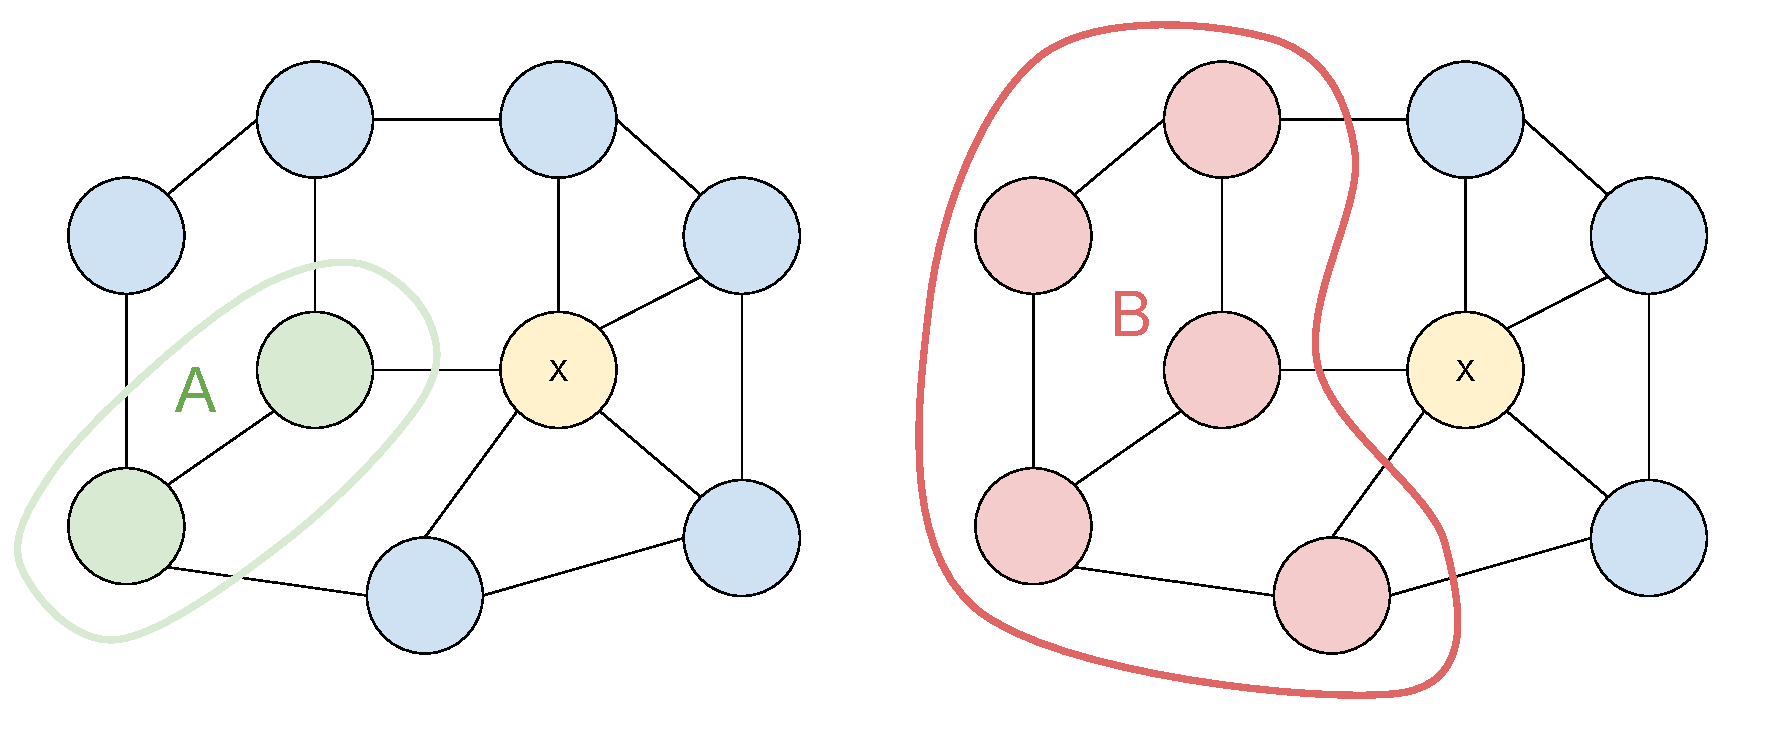
\includegraphics[scale=0.5]{sub.pdf}
\caption{Graphical representation of the cut function with two sets $A \subseteq B$ and a vertex $x \not\in B$.}\label{fig:graphAB}
\end{figure} By keeping this in mind, we can state that the rightmost part of \eqref{al:cutlast} is always at least as large as the leftmost part: specifically, the number of edges between $x$ and $B$ is at least as large as the number of edges between $x$ and $A$.

\QEDB


\section*{Exercise 6}
\subsection*{6.1}

In this section we will demonstrate that a symmetric matrix $A$ has only real eigenvalues $\lambda$ and orthogonal eigenvectos $x$~\cite{eigen}. Let us start from the definition of eigenvalues/eigenvectors:

\begin{align}\label{al:first}
A x = \lambda x
\end{align}
where its coniugate is:
\begin{align}\label{al:eigensym}
\bar{A} \bar{x} = \bar{\lambda} \bar{x}
\end{align}
Since $A$ is symmetric ($\bar{A} = A$), the last equation can be equivalently re-writed as:
\begin{align}\label{al:eigencmp}
A \bar{x} = \bar{\lambda} \bar{x}
\end{align}

Then we take the  transposition of the coniugate of the equation above (we remember that $A^T = A$ for symmetry):
\begin{align}
\bar{x}^T A = {\bar{x}}^T \bar{\lambda}
\end{align}
and we multiply both sides by $x$:
\begin{align}\label{eq:above}
\bar{x}^T A x = {\bar{x}}^T \bar{\lambda} x
\end{align}

By applying equation \eqref{al:first} to the left side of \eqref{eq:above} we get:
\begin{align}
\bar{x}^T \lambda x = {\bar{x}}^T \bar{\lambda} x
\end{align}
which is true iff $\lambda = \bar{\lambda}$ and consequently iff $\lambda$ is a real number.

Let us assume that we have two distinct eigenvalues $\lambda_1, \lambda_2$ and the corresponding eigenvectors $x_1, x_2$:
\begin{align}
A x_1 = \lambda_1 x_1\\
A x_2 = \lambda_2 x_2
\end{align}

Then, we apply both equations above into the following steps:
\begin{align}
x_1^T \lambda_1 x_2 = {(\lambda_1 x_1)}^T x_2 = {(A x_1)}^T x_2 = {x_1}^T A x_2 = {x_1}^T \lambda_2 x_2
\end{align}
which is true iff $\lambda_1 = \lambda_2$ or $x_1 x_2 = 0$: since we have originally assumed that $\lambda_1 \not= \lambda_2$, only the case with $x_1$ orthogonal to $x_2$ is applicable.

\QEDB



\subsection*{6.2}

In this section we will prove that, for any vector $x \in \mathbb{R}^{|V|}$ it is:

\begin{align}
x' L x = \frac{1}{d} \sum_{(u, v) \in E} (x_u - x_v)^2
\end{align}


First, we apply the definition of $L$ in $x' L x$:

\begin{align}
x' L x = x' (I - \frac{1}{d} A) x = x' x - \frac{1}{d} x' A x = \sum_{i = 1}^n {x^2_i} - \frac{1}{d} \sum_{i, j = 1}^n x_i x_j  a_{i, j}
\end{align}

Next, we cast the second sum into a sum over edges. We remember that, since the graph is undirected, the component $x_i x_j$ appears in the original sum twice ($(i, j)$ and $(j, i)$):

\begin{align}\label{al:prevsum}
\sum_{i = 1}^n {x^2_i} - \frac{1}{d} \sum_{(u, v) \in E} 2 x_u x_v = \sum_{i = 1}^n {x^2_i} - \frac{2}{d} \sum_{(u, v) \in E} x_u x_v
\end{align}

Then, we apply the same trick to the first sum. Similarly to the previous case, since the graph is $d$-regular, each $x_u^2$ will appear in the new sum $d$ times (while in \eqref{al:prevsum} it appears once):

\begin{align}\label{al:d}
\sum_{(u, v) \in E} \frac{1}{d}(x_u^2 + x_v^2) - \frac{1}{d} \sum_{(u, v) \in E} 2 x_u x_v
\end{align}

Finally, we can rewrite (\ref{al:d}) as follows:

\begin{align}
\frac{1}{d}\sum_{(u, v) \in E} (x_u^2 + x_v^2 - 2 x_u x_v) = \frac{1}{d}\sum_{(u, v) \in E} (x_u - x_v)^2  
\end{align}
\QEDB



\section*{Exercise 7}

\subsection*{7.1}

We define $P$ as the stochastic matrix where $p_{uv}~=~1/deg(u)$ and $\pi_u^t$ as the probability of being at vertex $u$ at time $t$. Our goal is to prove that the stationary distribution is proportional to the degree of nodes, namely $\pi_u^t = C \cdot deg(u)$, for $t \rightarrow +\infty$. Since the sum of probabilities has to be one, we have:
\begin{align}
\sum_{u \in V} \pi^t(u) = \sum_{u \in V} C \cdot deg(u) = 1 \iff C = \frac{1}{2m}\\
\end{align}
Then, we can prove that by performing a random walk with an initial distribution of
\begin{align} \label{al:unif}
\pi_u^0 = \frac{deg(u)}{2m}
\end{align}
 the probability to be in a vertex $u$ is proportional to its degree, independently from $t$.
 
First, we define a random walk as follows:
\begin{align}
\pi^{t + 1} = \pi^t P
\end{align}
Then, if we start from $\pi^0$ and we perform a ``random step'', we have that the probability of being in $u$ is:
\begin{align}
\pi_u^1 &= \sum_{(v, u) \in E} \pi_v^0\ p_{vu}\\
		&= \sum_{(v, u) \in E} \frac{deg(v)}{2m} \frac{1}{deg(v)}\\
		&= \sum_{(v, u) \in E} \frac{1}{2m}\\
        &= \frac{deg(u)}{2m}
\end{align}
Consequently, for each $u$, we will have $\pi_u^t = \deg(u) / 2m$  for each value of $t$. Therefore, the probability of being in $u$ after $t$ steps of our random walk is proportional to its degree.

\QEDB


On the other hand, this property does not hold for strongly connected-directed graphs. For example, in Figure~\ref{fig:graphprob} (on the left), the probability of being in nodes $[4, n]$ is lower than being in node $2$ (despite they have the same in- and out-degree). A random walker always passes on node $2$ in a path of length at least $3$, while this is not true for example, for node $4$.




\subsection*{7.2}

A strongly-connected directed graph in which a node has a a small in- and out-degree but a high probability of being visited in the random walk is represented in  Figure~\ref{fig:graphprob} (on the left). Despite of its low in- and out-degree, vertex $2$ has an high probability of being visited by a random walker: each random walk of length at least $3$ will always visit node $2$.


\begin{figure}
\centering
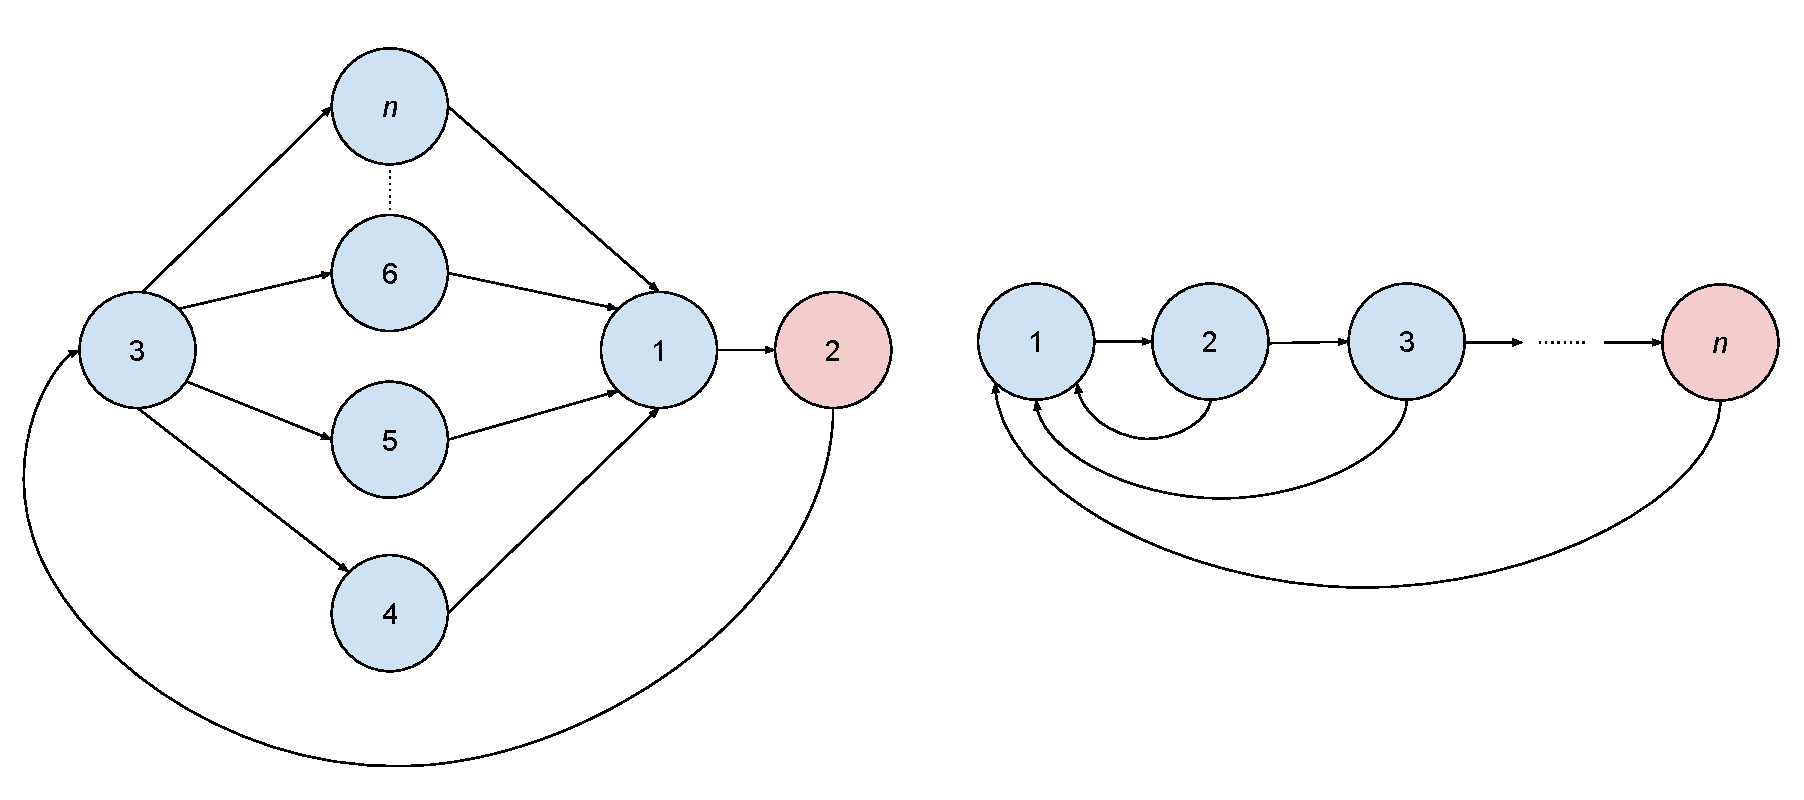
\includegraphics[scale=0.6]{graphs.pdf}
\caption{On the left, a graph where a node with a small degree and an high probability to be visited by a random walker exists (node $2$). On the right, a graph where a node with an exponentially small probability to be visited by a random walker exists (node $n$).}
\label{fig:graphprob}
\end{figure}



\subsection*{7.3}

A strongly-connected directed graph in which there is a vertex whose probability of being visited in random walk is exponentially small is represented in Figure \ref{fig:graphprob} (on the right). In detail, a random walker which starts from the node $1$ has a probability of $1/2^{n - 1}$ to end in the $n$-th vertex (after a random walk of length~$n - 1$).



\section*{Exercise 8}

This section is structured as follows. First, we will present a naive solution to the problem in question. Then, we will propose a faster algorithm by presenting and adapting to our context the solution describe in \cite{holm2001poly} to the Fully-dynamic Graph Connectivity Problem.

\subsection*{Naive Solution}
\begin{description}
\item[Algorithm.] A first naive solution can be the following. We use two data structures: an adjacent lists for representing the graph and a queue to quickly find the edge we have to remove at each step $T$.

At each step $T$, we add $e_T$ both into the adjacent lists and into the queue. Then, if $T > W$, we pop the edge from the head of the queue and we delete it from the adjacent lists. Finally, we perform a DFS-visit rooted from a random node in order to check if it reaches all other $n - 1$ nodes: if so,  $G(T, W)$ is connected, otherwise it is not connected.

Clearly, this solution presents three main advantages: (1) it is intuitive, (2) it is easy to implement and (3) it needs only of two basic data structures (adjacent lists and a queue). On the other hand, the query time of this algorithm needs a DFS-visit at each edge arrival.


\item[Space Complexity.] This algorithm needs $\mathcal{O}(n + W)$ space to represent the graph with adjacent~lists and the queue of edges.

\item[Update Time.] The update time of the adjacent lists costs $\mathcal{O}(1)$ to find the adjacent list of a node (by using an hash table) and $\mathcal{O}(1)$ to insert or remove the corresponding edge from the list:
\begin{itemize}
\item \textit{Insertion.} We are inserting the last (most recent) arrived edge, so we need to insert the edge at the end of the corresponding list. In detail, if we have to insert $(u, v)$ into our adjacent lists, we append $v$ (resp. $u$) to the list of $u$ (resp. $v$).
\item \textit{Deletion.} We are removing the oldest edge from the graph, so it will be the oldest edge from the corresponding list (the first element).  Similarly to the previous case, if we have to delete $(u, v)$ from our adjacent lists, we remove $v$ (resp. $u$) from the (head of the) list of $u$ (resp. $v$).
\end{itemize}

The update time of the queue is $\mathcal{O}(1)$. The output is given by performing a DFS-visit, which takes $\mathcal{O}(n + W)$ running time.

Summing up, the running time of the update procedure is owned by the DFS-visit: $\mathcal{O}(n + W)$.
\end{description}


\subsection*{Fast Solution}
In this section we present an adaptation of the solution presented in \cite{holm2001poly, mit, tor, stanford} applied to our context. First, we will present a well-known solution, originally presented in \cite{holm2001poly}, which uses a set of spanning forests in order to answer to connectivity queries in amortized $\mathcal{O}(\log_2^2 n)$ time. Then, we will describe how this solution can be adapted and used in our context, where a streaming model with sliding window is taken in into account.


\subsubsection*{Dynamic Graph Connectivity}

\cite{holm2001poly, mit, tor, stanford} describe a solution to the Fully-dynamic Graph Connectivity Problem, where the goal is to quickly check if two vertices belong to the same connected component of a graph that changes over the time. For the sake of simplicity, we will focus only on that parts of this algorithm that we need for solving this exercise and to understand how the solution proposed in the last section works.


The algorithm stores a set of hierarchically decomposed spanning forests, where edges are in different levels. The strategy of putting edges into lower levels is used as a charging scheme. The level of an edge seems not to have a ``real'' definition, but it simply is a quantity that changes over time. $G_i$ is the graph with edges $e$ such that $\text{level}(e) \leq i$. $F_i$ is the spanning forest of $G_i$ stored as an Euler-Tour tree (ET-tree) and $G = G_{\log_2 n}$. An ET-tree is an data structure used to represent a forest and which provides insertion and deletion in $\mathcal{O}(\log_2 n)$~\cite{stanford}. The algorithm we will present has two invariants:
\begin{enumerate}
\item Each connected component of $G_i$ has at most $2^i$ vertices: whenever we go down to a lower level, the max size of the connected components goes down by a factor of $2$.
\item  $F_0 \subseteq F_1 \subseteq \dots \subseteq F_{\log_2 n}$. Since the ``real'' spanning forest is $F_{\log_2 n}$, we can see $F_i$ as $F_{\log_2 n}$ restricted to $G_i$, namely $F_i = F_{\log_2 n} \cap G_i$.
\end{enumerate}

In order to understand the solution presented in the next section, we need to describe the following two operations:

\begin{itemize}
\item \textit{Insertion.} The insertion of an edge $e = (u, v)$ is performed (1) by setting the level of $e$ to $\log_2 n$ and then (2) by updating the adjacency lists of the graph with this new edge. Then, we perform an insertion into the corresponding ET-tree of $F_{\log_2 n}$: if $u$ and $v$ were disconnected in $F_{\log_2 n}$ they will be now connected in $F_{\log_2 n}$ after the insertion. Thanks to ET-tree, this operation is computed in $\mathcal{O}(\log_2 n)$.



\item \textit{Deletion.} The deletion of $e = (u, v)$ is performed as follows. First, we remove $e$ from the adjacency lists. Second, we distinguish two cases:

\begin{enumerate}
\item If $e \not\in F_{\log_2 n}$ then we have done, because invariant (2) this edge does not appear in the other $F_i$, with $i < \log_2 n$.
\item  On the other hand, if $e \in F_{\log_2 n}$ we proceed as follows. We delete $e$ from all $F_i$, for all $i \geq \text{level}(n)$. Then, we try to find a replacement edge, which is an edge which allows us to maintain the same connected components before the deletion.



For each level $i \in [\text{level}(e), \log_2 n]$ we have $T_u$ and $T_v$, which are the trees generated by deleting $e$: $T_u$ contains $u$ and $T_v$ contains $v$. Without loss of generality we assume $|T_v| \leq |T_u|$. Next, by applying invariant (1) we have that $|T_v| + |T_u| \leq 2^i$ and because $|T_v| \leq |T_u|$ we have that $|T_v| \leq 2^{i - 1}$. This means that we can afford to push the edges of $T_v$ down to level $i - 1$ (afford means that we would not destroy invariant (1)). If we want to find a replacement edge it seems that we have to scan all edges but, if we search from $T_v$, every edge that is useless decreases its level and gives us a ``free coin'' to continue (useful to have an amortized running time of $\mathcal{O}(\log_2 n)$). As long as we do not find the replacement edge, we push down the level of the considered edge, and we ``pay'' for it. Formally, we try to find the replacement edge as follows:

\begin{algorithm}[H]
\caption{Finding a replacement edge at level $i$.}\label{algo:replace}
\begin{algorithmic}[1]
\ForAll{$(x, y)\ \text{at level}\ i\ \text{with}\ x \in T_v$}
	\If{$y \in T_u$}
    	\State Add $(x, y)$ to $F_i, \dots, F_{\log_2 n}$
        \State \Return
    \Else
    	\State $\text{level}((x, y)) \leftarrow i - 1$
    \EndIf
\EndFor
\end{algorithmic}
\end{algorithm}

The amortized running time of this operation is proved to be $\mathcal{O}(\log_2^2 n)$ \cite{holm2001poly, mit, tor, stanford}. On the other hand, in order to efficiently perform this operation we need to augment our ET-trees, but it can be done by augment the trees with a constant amount of information per node~\cite{holm2001poly, mit, tor, stanford}.
\end{enumerate}

\end{itemize}


\subsubsection*{Graph Connectivity Detection in Streaming Model}

\begin{description}
\item[Algorithm.] The algorithm described in the previous section can be adapted to our problem as follows. We suppose to have a dynamic data structure $SF$, which owns our spanning forests $F_{\log_2 n}, \dots, F_0$ and which implements both \textit{Insertion} and \textit{Deletion} as described before. Additionally, we use the same queue described in \textit{Naive Solution} to quickly find the edge we have to remove at each step.

At each step $T$, we insert $e_T$ both into the queue and $SF$. Then, if $T > W$ we pop the edge from the head of the queue and we delete it from $SF$. Finally, we decide if the graph is connected whether the number of trees in $F_{\log_2 n} \in SF$ is one.

\item[Update Time] Whenever an edge arrives, we have to perform both an insertion and a deletion on our data structures. Clearly, the updating of the queue costs $\mathcal{O}(1)$, while the updating time of $SF$ costs $\mathcal{O}(\log_2^2 n)$ amortized running time. The number of trees in $F_{\log_2 n}$ is computed in $\mathcal{O}(1)$ time.

Summing up, the update time to decide the connectivity of the graph is  $\mathcal{O}(\log_2^2 n)$.

\item[Space Complexity.] The queue needs of $\mathcal{O}(W)$ space, while $SF$ is stored in $\mathcal{O}((n + W)\ \log_2 n)$ space: an adjacent lists for each $F_i$, with $i \in [0, \log_2 n]$.

Summing up, the whole space complexity is $\mathcal{O}((n + W) \log_2 n)$.
\end{description}





\section*{Acknowledgements}
I thank Manuele Sabbadin, Luca Pedrelli, Giulio Ermanno Pibiri, Massimiliano Bertolucci and Giovanna Broccia for the discussions about the problems addressed in this homework.


\begin{thebibliography}{100}

    
    \bibitem{mit}
    Erik Demaine, Josh Alman, Vlad Firoiu and Di Liu.
    \newblock Advanced Data Structures.
    \newblock \url{https://courses.csail.mit.edu/6.851/spring12/scribe/L20.pdf}

     \bibitem{tor}
    Camil Demetrescu, Irene Finocchi and Giuseppe F. Italiano.
    \newblock Dynamic Graphs.
    \newblock \url{http://www.diku.dk/PATH05/CRC-book1.pdf}

   \bibitem{flajolet1985probabilistic}
  Philippe Flajolet and G Nigel Martin.
  \newblock Probabilistic counting algorithms for data base applications.
  \newblock Journal of computer and system sciences, 1985.
 


	\bibitem{holm2001poly}
    Jacob Holm,  Kristian De Lichtenberg and Mikkel Thorup.
    \newblock Poly-logarithmic deterministic fully-dynamic algorithms for connectivity, minimum spanning tree, 2-edge, and biconnectivity.
    \newblock Journal of the ACM (JACM), 2001.

  \bibitem{lipkus1999proof}
  Alan H Lipkus.
  \newblock A proof of the triangle inequality for the Tanimoto distance.
  \newblock Journal of Mathematical Chemistry, 1999.
  

  \bibitem{palmer2002anf}
   Christopher R Palmer, Phillip B Gibbons, and Christos Faloutsos.
  \newblock ANF: A fast and scalable tool for data mining in massive graphs.
  \newblock Proceedings of the eighth ACM SIGKDD international conference on Knowledge discovery and data mining, 2002.
    

    
     \bibitem{stanford}
   Virginia V. Williams.
   \newblock Dynamic Graph Algorithms.
    \newblock \url{http://theory.stanford.edu/~virgi/cs267/lecture10.pdf}
    
    \bibitem{eigen}
  Dylan Zwick.
  \newblock Symmetric Matrices.
  \newblock \url{http://www.math.utah.edu/~zwick/Classes/Fall2012_2270/Lectures/Lecture32.pdf}
    
  
\end{thebibliography}


\end{document}